\documentclass[11pt]{article}
\usepackage[margin=1in]{geometry}
\usepackage{amsmath,amssymb}
\usepackage{graphicx}
\usepackage{booktabs}
\usepackage{hyperref}
\usepackage{natbib}
\usepackage{xcolor}
\usepackage{microtype}
\usepackage[affil-it]{authblk}
\usepackage[section]{placeins}

\newcommand{\TODO}[1]{\textcolor{red}{[TODO: #1]}}

% Extra space before floats (matches pQTL/cross-ancestry papers)
\setlength{\textfloatsep}{14pt plus 2pt minus 2pt}
\setlength{\intextsep}{10pt plus 2pt minus 2pt}

\title{A Graded Evaluation of RNA Structure Awareness\\in Foundation Models: From Stem--Loop Discrimination\\to Partner Specificity}

\author{Elliot Tower}
\affil{Independent researcher \\ \texttt{elliot@elliottower.ai}}
\date{}

% Running head for RNA journal (<=50 chars):
% Graded evaluation of RNA structure awareness

% Panel counts and every reported number, written by
% scripts/generate_results_tables.py from the stamped runs.
% Generated by scripts/generate_panel_description.py. Do not edit.
% Every figure below is computed from data/rfam_families/.
\newcommand{\panelN}{47}
\newcommand{\panelCurated}{52}
\newcommand{\panelWithdrawn}{5}
\newcommand{\panelClasses}{riboswitches (14), cis-regulatory elements (8), other ncRNAs (8), ribozymes (6), miRNA precursors (4), snRNAs (4), tRNAs (2), and CRISPR repeats (1)}
\newcommand{\panelLengthRange}{30--387}
\newcommand{\panelLengthMedian}{106}
\newcommand{\panelLengthIQR}{77.5--166}
\newcommand{\panelStemGC}{59.1}
\newcommand{\panelLoopGC}{43.0}
\newcommand{\panelGCEnriched}{40}
\newcommand{\panelGCScored}{47}

% Written by scripts/generate_results_tables.py. Do not edit.
\newcommand{\confirmatoryN}{36}
\newcommand{\gateThreshold}{8}
\newcommand{\gateRegistered}{7}
\newcommand{\bootstrapB}{10{,}000}
\newcommand{\panelHashShort}{\texttt{5c4d6f6d4c32}}
\newcommand{\provenanceRuns}{17}
\newcommand{\provenanceCommits}{2}
\newcommand{\provenanceStacks}{5}
\newcommand{\ratioErnieRNA}{1.276}
\newcommand{\ciErnieRNA}{[1.22, 1.34]}
\newcommand{\exceedErnieRNA}{31}
\newcommand{\dinucErnieRNA}{30}
\newcommand{\retainErnieRNA}{30 of 31}
\newcommand{\retainPctErnieRNA}{97\%}
\newcommand{\probeErnieRNA}{0.683}
\newcommand{\probeDeltaErnieRNA}{+0.183}
\newcommand{\probeLayerErnieRNA}{11}
\newcommand{\attnErnieRNA}{0.113}
\newcommand{\psErnieRNA}{0.1113}
\newcommand{\gateErnieRNA}{34/36}
\newcommand{\gateCountErnieRNA}{34}
\newcommand{\eligibleErnieRNA}{36}
\newcommand{\nullErnieRNA}{32/34}
\newcommand{\consErnieRNA}{32/34}
\newcommand{\hthreeErnieRNA}{0.885}
\newcommand{\psPeakErnieRNA}{12}
\newcommand{\psLayersErnieRNA}{13}
\newcommand{\psPeakCountErnieRNA}{29 of 34}
\newcommand{\ratioRiNALMo}{1.143}
\newcommand{\ciRiNALMo}{[1.12, 1.17]}
\newcommand{\exceedRiNALMo}{17}
\newcommand{\dinucRiNALMo}{15}
\newcommand{\retainRiNALMo}{15 of 17}
\newcommand{\retainPctRiNALMo}{88\%}
\newcommand{\probeRiNALMo}{0.633}
\newcommand{\probeDeltaRiNALMo}{+0.133}
\newcommand{\probeLayerRiNALMo}{32}
\newcommand{\attnRiNALMo}{0.107}
\newcommand{\psRiNALMo}{0.2062}
\newcommand{\gateRiNALMo}{32/36}
\newcommand{\gateCountRiNALMo}{32}
\newcommand{\eligibleRiNALMo}{36}
\newcommand{\nullRiNALMo}{31/32}
\newcommand{\consRiNALMo}{29/32}
\newcommand{\hthreeRiNALMo}{0.886}
\newcommand{\psPeakRiNALMo}{33}
\newcommand{\psLayersRiNALMo}{34}
\newcommand{\psPeakCountRiNALMo}{31 of 32}
\newcommand{\ratioRNAFM}{1.722}
\newcommand{\ciRNAFM}{[1.53, 1.95]}
\newcommand{\exceedRNAFM}{0}
\newcommand{\dinucRNAFM}{0}
\newcommand{\probeRNAFM}{0.550}
\newcommand{\probeDeltaRNAFM}{+0.050}
\newcommand{\probeLayerRNAFM}{0}
\newcommand{\attnRNAFM}{0.049}
\newcommand{\psRNAFM}{$8.9 \times 10^{-5}$}
\newcommand{\gateRNAFM}{2/36}
\newcommand{\gateCountRNAFM}{2}
\newcommand{\eligibleRNAFM}{36}
\newcommand{\nullRNAFM}{0/2}
\newcommand{\consRNAFM}{0/2}
\newcommand{\hthreeRNAFM}{0.250}
\newcommand{\psPeakRNAFM}{1}
\newcommand{\psLayersRNAFM}{13}
\newcommand{\psPeakCountRNAFM}{1 of 2}
\newcommand{\ratioUTRLM}{1.056}
\newcommand{\ciUTRLM}{[1.04, 1.08]}
\newcommand{\exceedUTRLM}{3}
\newcommand{\dinucUTRLM}{2}
\newcommand{\retainUTRLM}{2 of 3}
\newcommand{\retainPctUTRLM}{67\%}
\newcommand{\probeUTRLM}{0.578}
\newcommand{\probeDeltaUTRLM}{+0.078}
\newcommand{\probeLayerUTRLM}{1}
\newcommand{\attnUTRLM}{0.051}
\newcommand{\psUTRLM}{$8.3 \times 10^{-6}$}
\newcommand{\gateUTRLM}{27/36}
\newcommand{\gateCountUTRLM}{27}
\newcommand{\eligibleUTRLM}{36}
\newcommand{\nullUTRLM}{18/27}
\newcommand{\consUTRLM}{4/27}
\newcommand{\hthreeUTRLM}{0.215}
\newcommand{\psPeakUTRLM}{0}
\newcommand{\psLayersUTRLM}{7}
\newcommand{\psPeakCountUTRLM}{15 of 27}
\newcommand{\ratioSpliceBERT}{1.040}
\newcommand{\ciSpliceBERT}{[1.03, 1.05]}
\newcommand{\exceedSpliceBERT}{3}
\newcommand{\dinucSpliceBERT}{1}
\newcommand{\retainSpliceBERT}{1 of 3}
\newcommand{\retainPctSpliceBERT}{33\%}
\newcommand{\probeSpliceBERT}{0.566}
\newcommand{\probeDeltaSpliceBERT}{+0.066}
\newcommand{\probeLayerSpliceBERT}{1}
\newcommand{\attnSpliceBERT}{0.054}
\newcommand{\psSpliceBERT}{0.0002}
\newcommand{\gateSpliceBERT}{25/36}
\newcommand{\gateCountSpliceBERT}{25}
\newcommand{\eligibleSpliceBERT}{36}
\newcommand{\nullSpliceBERT}{15/25}
\newcommand{\consSpliceBERT}{4/25}
\newcommand{\hthreeSpliceBERT}{0.270}
\newcommand{\psPeakSpliceBERT}{0}
\newcommand{\psLayersSpliceBERT}{7}
\newcommand{\psPeakCountSpliceBERT}{11 of 25}
\newcommand{\ratioNTvTwo}{1.113}
\newcommand{\ciNTvTwo}{[1.08, 1.14]}
\newcommand{\exceedNTvTwo}{15}
\newcommand{\dinucNTvTwo}{10}
\newcommand{\retainNTvTwo}{10 of 15}
\newcommand{\retainPctNTvTwo}{67\%}
\newcommand{\probeNTvTwo}{0.531}
\newcommand{\probeDeltaNTvTwo}{+0.031}
\newcommand{\probeLayerNTvTwo}{7}
\newcommand{\attnNTvTwo}{0.242}
\newcommand{\psNTvTwo}{0.0014}
\newcommand{\gateNTvTwo}{1/4}
\newcommand{\gateCountNTvTwo}{1}
\newcommand{\eligibleNTvTwo}{4}
\newcommand{\nullNTvTwo}{0/1}
\newcommand{\consNTvTwo}{0/1}
\newcommand{\hthreeNTvTwo}{0.500}
\newcommand{\psPeakNTvTwo}{0}
\newcommand{\psLayersNTvTwo}{13}
\newcommand{\psPeakCountNTvTwo}{1 of 1}
\newcommand{\ratioDNABERTTwo}{1.003}
\newcommand{\ciDNABERTTwo}{[0.97, 1.04]}
\newcommand{\exceedDNABERTTwo}{8}
\newcommand{\dinucDNABERTTwo}{5}
\newcommand{\retainDNABERTTwo}{5 of 8}
\newcommand{\retainPctDNABERTTwo}{62\%}
\newcommand{\probeDNABERTTwo}{0.530}
\newcommand{\probeDeltaDNABERTTwo}{+0.030}
\newcommand{\probeLayerDNABERTTwo}{1}
\newcommand{\attnDNABERTTwo}{0.199}
\newcommand{\psDNABERTTwo}{-0.0680}
\newcommand{\gateDNABERTTwo}{0/8}
\newcommand{\gateCountDNABERTTwo}{0}
\newcommand{\eligibleDNABERTTwo}{8}
\newcommand{\ratioHyenaDNA}{1.160}
\newcommand{\ciHyenaDNA}{[1.12, 1.20]}
\newcommand{\exceedHyenaDNA}{8}
\newcommand{\dinucHyenaDNA}{7}
\newcommand{\retainHyenaDNA}{7 of 8}
\newcommand{\retainPctHyenaDNA}{88\%}
\newcommand{\probeHyenaDNA}{0.577}
\newcommand{\probeDeltaHyenaDNA}{+0.077}
\newcommand{\probeLayerHyenaDNA}{0}
\newcommand{\psHyenaDNA}{0.0002}
\newcommand{\gateHyenaDNA}{27/36}
\newcommand{\gateCountHyenaDNA}{27}
\newcommand{\eligibleHyenaDNA}{36}
\newcommand{\nullHyenaDNA}{13/27}
\newcommand{\consHyenaDNA}{6/27}
\newcommand{\hthreeHyenaDNA}{0.162}
\newcommand{\psPeakHyenaDNA}{0}
\newcommand{\psLayersHyenaDNA}{4}
\newcommand{\psPeakCountHyenaDNA}{26 of 27}
\newcommand{\ratioCaduceus}{1.206}
\newcommand{\ciCaduceus}{[1.16, 1.26]}
\newcommand{\exceedCaduceus}{8}
\newcommand{\dinucCaduceus}{4}
\newcommand{\retainCaduceus}{4 of 8}
\newcommand{\retainPctCaduceus}{50\%}
\newcommand{\probeCaduceus}{0.577}
\newcommand{\probeDeltaCaduceus}{+0.077}
\newcommand{\probeLayerCaduceus}{0}
\newcommand{\psCaduceus}{0.0039}
\newcommand{\gateCaduceus}{18/36}
\newcommand{\gateCountCaduceus}{18}
\newcommand{\eligibleCaduceus}{36}
\newcommand{\nullCaduceus}{13/18}
\newcommand{\consCaduceus}{8/18}
\newcommand{\hthreeCaduceus}{0.402}
\newcommand{\psPeakCaduceus}{3}
\newcommand{\psLayersCaduceus}{17}
\newcommand{\psPeakCountCaduceus}{4 of 18}
\newcommand{\ratioEvo}{1.450}
\newcommand{\ciEvo}{[1.30, 1.63]}
\newcommand{\exceedEvo}{8}
\newcommand{\dinucEvo}{6}
\newcommand{\retainEvo}{6 of 8}
\newcommand{\retainPctEvo}{75\%}
\newcommand{\probeEvo}{0.552}
\newcommand{\probeDeltaEvo}{+0.052}
\newcommand{\probeLayerEvo}{0}
\newcommand{\psEvo}{0.0017}
\newcommand{\gateEvo}{13/36}
\newcommand{\gateCountEvo}{13}
\newcommand{\eligibleEvo}{36}
\newcommand{\nullEvo}{6/13}
\newcommand{\consEvo}{2/13}
\newcommand{\hthreeEvo}{0.376}
\newcommand{\psPeakEvo}{12}
\newcommand{\psLayersEvo}{32}
\newcommand{\psPeakCountEvo}{7 of 13}
\newcommand{\exceedUntrainedErnieRNA}{2}
\newcommand{\ratioUntrainedErnieRNA}{1.815}
\newcommand{\retainUntrainedErnieRNA}{2 of 2}
\newcommand{\attnUntrainedErnieRNA}{0.085}
\newcommand{\attnDeltaErnieRNA}{+0.027}
\newcommand{\attnFamilyDeltaErnieRNA}{+0.027}
\newcommand{\attnHigherTrainedErnieRNA}{47}
\newcommand{\attnHigherUntrainedErnieRNA}{0}
\newcommand{\psUntrainedErnieRNA}{$6.0 \times 10^{-9}$}
\newcommand{\gateUntrainedErnieRNA}{6/36}
\newcommand{\nullUntrainedErnieRNA}{4/6}
\newcommand{\signErnieRNA}{7/47}
\newcommand{\signPctErnieRNA}{15\%}
\newcommand{\exceedUntrainedRiNALMo}{5}
\newcommand{\ratioUntrainedRiNALMo}{4.556}
\newcommand{\retainUntrainedRiNALMo}{1 of 5}
\newcommand{\attnUntrainedRiNALMo}{0.064}
\newcommand{\attnDeltaRiNALMo}{+0.044}
\newcommand{\attnFamilyDeltaRiNALMo}{+0.044}
\newcommand{\attnHigherTrainedRiNALMo}{46}
\newcommand{\attnHigherUntrainedRiNALMo}{1}
\newcommand{\psUntrainedRiNALMo}{$1.1 \times 10^{-8}$}
\newcommand{\gateUntrainedRiNALMo}{6/36}
\newcommand{\nullUntrainedRiNALMo}{4/6}
\newcommand{\signRiNALMo}{0/47}
\newcommand{\signPctRiNALMo}{0\%}
\newcommand{\exceedUntrainedRNAFM}{2}
\newcommand{\ratioUntrainedRNAFM}{2.257}
\newcommand{\retainUntrainedRNAFM}{1 of 2}
\newcommand{\attnUntrainedRNAFM}{0.043}
\newcommand{\attnDeltaRNAFM}{+0.006}
\newcommand{\attnFamilyDeltaRNAFM}{+0.006}
\newcommand{\attnHigherTrainedRNAFM}{33}
\newcommand{\attnHigherUntrainedRNAFM}{14}
\newcommand{\psUntrainedRNAFM}{$4.5 \times 10^{-9}$}
\newcommand{\gateUntrainedRNAFM}{9/36}
\newcommand{\nullUntrainedRNAFM}{5/9}
\newcommand{\signRNAFM}{17/47}
\newcommand{\signPctRNAFM}{36\%}
\newcommand{\exceedUntrainedUTRLM}{1}
\newcommand{\ratioUntrainedUTRLM}{1.038}
\newcommand{\retainUntrainedUTRLM}{0 of 1}
\newcommand{\attnUntrainedUTRLM}{0.054}
\newcommand{\attnDeltaUTRLM}{-0.003}
\newcommand{\attnFamilyDeltaUTRLM}{-0.003}
\newcommand{\attnHigherTrainedUTRLM}{16}
\newcommand{\attnHigherUntrainedUTRLM}{31}
\newcommand{\psUntrainedUTRLM}{$-2.0 \times 10^{-8}$}
\newcommand{\gateUntrainedUTRLM}{4/36}
\newcommand{\nullUntrainedUTRLM}{0/4}
\newcommand{\signUTRLM}{31/47}
\newcommand{\signPctUTRLM}{66\%}
\newcommand{\exceedUntrainedSpliceBERT}{4}
\newcommand{\ratioUntrainedSpliceBERT}{1.238}
\newcommand{\retainUntrainedSpliceBERT}{4 of 4}
\newcommand{\attnUntrainedSpliceBERT}{0.032}
\newcommand{\attnDeltaSpliceBERT}{+0.022}
\newcommand{\attnFamilyDeltaSpliceBERT}{+0.022}
\newcommand{\attnHigherTrainedSpliceBERT}{45}
\newcommand{\attnHigherUntrainedSpliceBERT}{2}
\newcommand{\psUntrainedSpliceBERT}{$7.1 \times 10^{-10}$}
\newcommand{\gateUntrainedSpliceBERT}{9/36}
\newcommand{\nullUntrainedSpliceBERT}{5/9}
\newcommand{\signSpliceBERT}{10/47}
\newcommand{\signPctSpliceBERT}{21\%}
\newcommand{\exceedUntrainedNTvTwo}{10}
\newcommand{\ratioUntrainedNTvTwo}{1.037}
\newcommand{\retainUntrainedNTvTwo}{9 of 10}
\newcommand{\attnUntrainedNTvTwo}{0.246}
\newcommand{\attnDeltaNTvTwo}{-0.004}
\newcommand{\attnFamilyDeltaNTvTwo}{-0.004}
\newcommand{\attnHigherTrainedNTvTwo}{23}
\newcommand{\attnHigherUntrainedNTvTwo}{24}
\newcommand{\psUntrainedNTvTwo}{$-7.5 \times 10^{-9}$}
\newcommand{\gateUntrainedNTvTwo}{1/4}
\newcommand{\nullUntrainedNTvTwo}{0/1}
\newcommand{\signNTvTwo}{40/47}
\newcommand{\signPctNTvTwo}{85\%}
\newcommand{\exceedUntrainedDNABERTTwo}{6}
\newcommand{\ratioUntrainedDNABERTTwo}{8.416}
\newcommand{\retainUntrainedDNABERTTwo}{4 of 6}
\newcommand{\attnUntrainedDNABERTTwo}{0.190}
\newcommand{\attnDeltaDNABERTTwo}{+0.009}
\newcommand{\attnFamilyDeltaDNABERTTwo}{+0.009}
\newcommand{\attnHigherTrainedDNABERTTwo}{27}
\newcommand{\attnHigherUntrainedDNABERTTwo}{20}
\newcommand{\psUntrainedDNABERTTwo}{-0.0026}
\newcommand{\gateUntrainedDNABERTTwo}{2/8}
\newcommand{\nullUntrainedDNABERTTwo}{0/2}
\newcommand{\signDNABERTTwo}{27/47}
\newcommand{\signPctDNABERTTwo}{57\%}
\newcommand{\domainRankBiserial}{+0.04}
\newcommand{\domainP}{1.000}
\newcommand{\familiesScored}{47}
\newcommand{\expectedFalsePositives}{2.4}
\newcommand{\tuPerFamilyRNAFM}{0.93}
\newcommand{\tuOfMeansRNAFM}{0.76}
\newcommand{\tuPerFamilyRiNALMo}{0.50}
\newcommand{\tuOfMeansRiNALMo}{0.25}
\newcommand{\tuPerFamilySpliceBERT}{0.87}
\newcommand{\tuOfMeansSpliceBERT}{0.84}
\newcommand{\transversionAlphabet}{A$\to$C, C$\to$A, G$\to$U, U$\to$C}
\newcommand{\transErnieRNA}{1.253}
\newcommand{\transDeltaErnieRNA}{-1.7\%}
\newcommand{\transRiNALMo}{1.144}
\newcommand{\transDeltaRiNALMo}{+0.1\%}
\newcommand{\transRNAFM}{1.701}
\newcommand{\transDeltaRNAFM}{-1.2\%}
\newcommand{\transUTRLM}{1.058}
\newcommand{\transDeltaUTRLM}{+0.2\%}
\newcommand{\transSpliceBERT}{1.051}
\newcommand{\transDeltaSpliceBERT}{+1.0\%}
\newcommand{\transNTvTwo}{1.124}
\newcommand{\transDeltaNTvTwo}{+1.0\%}
\newcommand{\transDNABERTTwo}{0.988}
\newcommand{\transDeltaDNABERTTwo}{-1.5\%}
\newcommand{\transHyenaDNA}{1.073}
\newcommand{\transDeltaHyenaDNA}{-7.5\%}
\newcommand{\transCaduceus}{1.158}
\newcommand{\transDeltaCaduceus}{-4.0\%}
\newcommand{\transEvo}{1.465}
\newcommand{\transDeltaEvo}{+1.0\%}
\newcommand{\transversionWidest}{HyenaDNA}
\newcommand{\transversionWidestDeviation}{7.5\%}
\newcommand{\transversionBound}{8\%}
\newcommand{\attnBound}{0.05}
\newcommand{\attnWidest}{RiNALMo}
\newcommand{\attnWidestFactor}{1.7}
\newcommand{\psSeparation}{29}


\begin{document}
\maketitle

\noindent\textbf{Keywords:} RNA foundation models, secondary structure, composition confound, partner specificity, evaluation framework, perturbation analysis

% ============================================================================
% ABSTRACT — ~200 words
% Sequence: problem, design, primary result, positive result, replication,
%           interpretation, scope
% ============================================================================
\begin{abstract}
Evaluating whether RNA foundation models encode base-pairing structure requires
separating learned representation from nucleotide composition. Stems are GC-rich
and loops are AU-rich, so any composition-sensitive embedding inherits that
enrichment as apparent structure awareness. We apply a three-rung ladder to ten
RNA- and DNA-pretrained models across \panelN{} Rfam families. A
nucleotide-stratified null absorbs most of the apparent signal at Rung~1; a
dinucleotide-preserving null at Rung~2 leaves ERNIE-RNA with 30 families and
RiNALMo with 15, and every other model with fewer than nine. At Rung~3 a
mutation must perturb its base-pairing partner more than that partner's own stem
neighbours, measured against a null that permutes partner assignments within
each stem. Two models resolve which position pairs with which: RiNALMo at
$0.872$ per-pair precision and ERNIE-RNA at $0.888$, where that null puts chance
at $0.102$ and $0.124$. Three more exceed their own chance rates by an order of
magnitude less---Caduceus by $0.122$, RNA-FM by $0.109$---and the remaining five
are at chance. Pretraining domain does not order the panel: Caduceus is a 14M
DNA-pretrained model and outscores three of the five RNA-pretrained ones.
A randomly initialized ERNIE-RNA clears every rung, reaching $0.490$ per-pair
precision. Its architecture holds a hardcoded Watson--Crick table in a buffer
that weight randomization does not reach; ablating it drops the randomly
initialized model to its own chance rate, $+0.012$ excess, while the trained
model retains $+0.725$.
\end{abstract}

% ============================================================================
% INTRODUCTION — 5 paragraphs, ~800 words
% Sequence: why it matters, confound, gap, what we do, contributions
% ============================================================================
\section{Introduction}
\label{sec:intro}

% P1: Why this matters
RNA foundation models are routinely claimed to encode secondary structure,
but the evaluation methods---downstream task performance, linear probing,
mutation sensitivity, attention--contact correlation---each answer different
questions, and none controls for sequence composition. Deep learning models
for RNA structure prediction may fail to generalize across families
\citep{szikszai2022generalization}; whether the same fragility applies to
learned representations has received less scrutiny.

% P2: The specific confound
Stems and loops differ in sequence composition. Across \panelN{} Rfam families,
stems average 59.7\% G/C content while loops average 45.6\%---a 14.1
percentage-point enrichment (Figure~\ref{fig:composition}). Because complement swaps at G/C positions
produce inherently larger embedding perturbations than at A/U positions,
any naive stem-versus-loop comparison inherits this enrichment. A
representation can therefore separate stems from loops without encoding
pairing topology.

% P3: The gap
Each evaluation method inherits the composition confound differently.
Linear probes can classify stems from loops using GC content alone.
Mutation sensitivity ratios conflate the larger perturbation magnitude at
G/C sites with structural relevance. Attention--contact correlations
bypass embeddings entirely and so measure a different channel. To
distinguish composition sensitivity from structure awareness, an
evaluation must control for nucleotide identity while testing whether
perturbations propagate to specific pairing partners.

% P4: What this study does — rung framing
These observations motivate a graded evaluation.
``Structure awareness'' encompasses at least three levels of
resolution, each demanding stronger knowledge: (1)~stem-versus-loop
discrimination, achievable by any representation sensitive to
nucleotide composition; (2)~discrimination surviving composition
controls at one and two orders of sequence context; and (3)~knowing
which specific position pairs with which, requiring that the model
encode the pairing topology. We apply this three-rung ladder to ten models across five architectures
and three orders of magnitude in parameter count.

% P5: Contributions + closing
The evaluation reveals a surprising asymmetry: the hardest test
produces the clearest positive result. Two RNA-pretrained
models---ERNIE-RNA (86M, with an architectural base-pairing attention
bias) and RiNALMo (650M, standard attention)---clear Rung~3 with
partner specificity two orders of magnitude above all other models,
while the remaining eight produce near-zero signal. We contribute:
(1)~a composition-controlled perturbation evaluation for RNA
foundation models; (2)~a ten-model benchmark with randomized-weight
controls on \panelN{} Rfam families; and (3)~evidence that two models
retain partner-specific pairing responses after composition controls are
applied.


% ============================================================================
% RESULTS — inferential logic: confound first, positive result, replication,
%           robustness, HTT last
% ============================================================================
\section{Results}

\subsection{Composition creates apparent structure signal (Rungs 1--2)}
\label{sec:composition-results}

Mutating a position to its Watson--Crick complement perturbs stem positions
more than loop positions in nine of ten models, with mean ratios from
$\ratioRNAFM{}$ (RNA-FM) down to near unity (Table~\ref{tab:rung1}). Stems in
this panel are GC-rich and loops are AU-rich---mean stem GC $\panelStemGC{}\%$
against loop GC $\panelLoopGC{}\%$---so a ratio above one is what a
composition-sensitive embedding produces whether or not it represents pairing.

Against a null that permutes stem and loop labels within nucleotide strata, most
of that signal is absorbed. At $\alpha = 0.05$ per family, chance alone places
2.4 of $\panelN{}$ families above the 95th percentile. ERNIE-RNA exceeds it in
$\exceedErnieRNA{}$ families and RiNALMo in $\exceedRiNALMo{}$; RNA-FM, whose
raw ratio is the largest in the panel, exceeds it in $\exceedRNAFM{}$.

A ratio and a composition-controlled count therefore order the models
differently, and neither distinguishes a model that tracks pairing from one that
tracks the nucleotides pairing implies. Rung 2 tightens the null to preserve
dinucleotide composition; Rung 3 changes the question.

\begin{figure}[htbp]
\centering
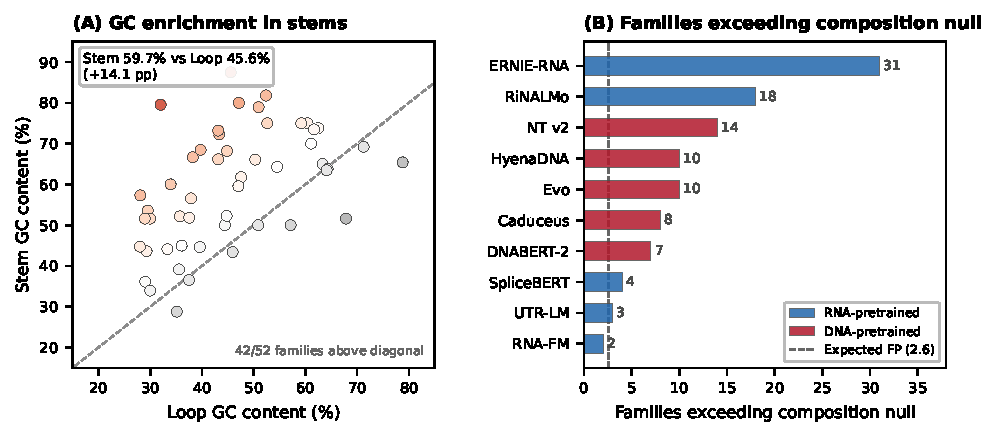
\includegraphics[width=\textwidth]{../figures/figure2_composition.pdf}
\caption{Composition confound. (A)~Stem GC content exceeds loop GC content
in \panelGCEnriched{} of \panelGCScored{} families (mean stem GC
\panelStemGC{}\% against loop GC \panelLoopGC{}\%). (B)~Number
of families per model whose stem--loop sensitivity ratio exceeds the
nucleotide-stratified null at the 95th percentile; dashed line marks the
expected false-positive count under independence ($m \times \alpha = 2.6$).
ERNIE-RNA (31) and RiNALMo (18) retain the most signal after composition
control.}
\label{fig:composition}
\end{figure}


\subsection{Probe validation}
\label{sec:probe-validation}

Eight of ten models score at their own chance rate at Rung 3, which admits two
readings the panel cannot separate, since every arm in it is a model under test.
We therefore run the Rung 3 procedure unchanged on two constructed embeddings
whose answer is fixed in advance. In the oracle, each position's representation
is a function of its own nucleotide and its partner's; in the local control, of
its own nucleotide and its two sequence neighbours.

The oracle reaches per-pair precision $1.000$ against a derangement chance rate
of $0.099$. The local control reaches $0.155$ against $0.173$. Both use the same
statistic, the same null and the same code path as every model in
Table~\ref{tab:rung3}, over the $\chanceRateN{}$ families of the Rung 3
analysis set.

The two chance rates differ, $0.099$ and $0.173$, on systems whose answers are
known.

\subsection{Partner specificity separates two models (Rung 3)}
\label{sec:ps-results}

\begin{table}[htbp]
\centering
\caption{Mutation sensitivity across ten models on the repaired panel
($N = \panelN{}$ Rfam families). Bootstrap 95\% CIs on the mean ratio
resample per-family ratios ($B = 10{,}000$).
At $\alpha = 0.05$ per family, 2.4 of 47
families are expected to exceed the null by chance. Attention $\rho$ is the mean
best-head-best-layer Spearman correlation between symmetrized attention and the
contact map, and is undefined for the three state-space models. Probing $\Delta$
is balanced accuracy minus 0.5. Untrained rows randomize every weight at a fixed
seed and load through the same adapter as the trained row above them.}
\label{tab:rung1}
\small
\begin{tabular}{lrlccc}
\toprule
\textbf{Model} & \textbf{Mean ratio} & \textbf{95\% CI} & \textbf{Fam $>$ null} & \textbf{Attn $\rho$} & \textbf{Probing $\Delta$} \\
\midrule
ERNIE-RNA (86M, RNA)       & 1.276 & [1.22, 1.34] & 31/47 & 0.113 & $+0.183$ \\
RiNALMo (650M, RNA)        & 1.143 & [1.12, 1.17] & 17/47 & 0.107 & $+0.134$ \\
RNA-FM (99M, RNA)          & 1.741 & [1.53, 1.98] & 0/47 & 0.048 & $+0.050$ \\
UTR-LM ($\sim$2M, RNA)     & 1.056 & [1.04, 1.08] & 3/47 & 0.051 & $+0.078$ \\
SpliceBERT (19M, RNA)      & 1.040 & [1.03, 1.05] & 3/47 & 0.054 & $+0.066$ \\
NT~v2 (56M, DNA)           & 1.098 & [1.08, 1.12] & 9/47 & 0.234 & $+0.036$ \\
DNABERT-2 (117M, DNA)      & 0.996 & [0.98, 1.01] & 3/47 & 0.196 & $+0.051$ \\
HyenaDNA (5.4M, DNA)       & 1.160 & [1.12, 1.20] & 8/47 & --- & $+0.077$ \\
Caduceus (14M, DNA)        & 1.206 & [1.16, 1.26] & 8/47 & --- & $+0.077$ \\
Evo (7B, DNA)              & 1.458 & [1.30, 1.64] & 8/47 & --- & $+0.052$ \\
\midrule
ERNIE-RNA untrained        & 1.164 & [1.12, 1.21] & 10/47 & 0.085 & $+0.044$ \\
RiNALMo untrained          & 1.156 & [1.13, 1.19] & 10/47 & 0.064 & $+0.077$ \\
RNA-FM untrained           & 1.043 & [1.04, 1.05] & 3/47 & 0.043 & $+0.073$ \\
UTR-LM untrained           & 1.038 & [1.03, 1.04] & 1/47 & 0.054 & $+0.077$ \\
SpliceBERT untrained       & 1.054 & [1.04, 1.07] & 0/47 & 0.032 & $+0.070$ \\
NT~v2 untrained            & 1.015 & [1.01, 1.02] & 5/47 & 0.241 & $+0.025$ \\
DNABERT-2 untrained        & 33.880 & [0.95, 93.92] & 6/47 & 0.153 & $+0.011$ \\
\bottomrule
\end{tabular}
\end{table}


\begin{table}[htbp]
\centering
\caption{Dinucleotide-stratified null across all models on the repaired panel.
``Fam $>$ nuc'' counts families exceeding the nucleotide-stratified null;
``Survive dinuc'' counts how many of those also exceed the
dinucleotide-stratified null, which is computed only where the first-order null
is exceeded. Retention is the second count over the first, and its bootstrap
95\% CI resamples the families in the first.}
\label{tab:rung2}
\small
\begin{tabular}{lrrll}
\toprule
\textbf{Model} & \textbf{Fam $>$ nuc} & \textbf{Survive dinuc} & \textbf{Retention} & \textbf{95\% CI} \\
\midrule
ERNIE-RNA (86M, RNA)       & 31 & 30 & 97\% & [0.90, 1.00] \\
RiNALMo (650M, RNA)        & 17 & 15 & 88\% & [0.71, 1.00] \\
NT~v2 (56M, DNA)           & 15 & 10 & 67\% & [0.40, 0.87] \\
DNABERT-2 (117M, DNA)      & 8 & 5 & 62\% & [0.25, 1.00] \\
HyenaDNA (5.4M, DNA)       & 8 & 7 & 88\% & [0.62, 1.00] \\
Caduceus (14M, DNA)        & 8 & 4 & 50\% & [0.12, 0.88] \\
Evo (7B, DNA)              & 8 & 6 & 75\% & [0.38, 1.00] \\
UTR-LM ($\sim$2M, RNA)     & 3 & 2 & 67\% & [0.00, 1.00] \\
SpliceBERT (19M, RNA)      & 3 & 1 & 33\% & [0.00, 1.00] \\
RNA-FM (99M, RNA)          & 0 & 0 & --- & --- \\
\midrule
ERNIE-RNA untrained        & 2 & 2 & 100\% & [1.00, 1.00] \\
RiNALMo untrained          & 5 & 1 & 20\% & [0.00, 0.60] \\
RNA-FM untrained           & 2 & 1 & 50\% & [0.00, 1.00] \\
UTR-LM untrained           & 1 & 0 & 0\% & [0.00, 0.00] \\
SpliceBERT untrained       & 4 & 4 & 100\% & [1.00, 1.00] \\
NT~v2 untrained            & 10 & 9 & 90\% & [0.70, 1.00] \\
DNABERT-2 untrained        & 6 & 4 & 67\% & [0.33, 1.00] \\
\bottomrule
\end{tabular}
\end{table}


\begin{table}[htbp]
\centering
\caption{Perturbation specificity on the repaired panel. 38 of \panelN{} families qualify ($\geq 15$ WC pairs with $\geq 3$ per stem); the two pilot families are quarantined, leaving $N = 36$ confirmatory families. Mean PS is taken over those $N$. Gate counts families passing the stem-versus-loop positive control, and the two null columns are computed among gate-passing families: $>$~null is the primary within-stem derangement null and $>$~cons.\ the conservative variant, reported together because the registration defines both. H3 precision is the mean of per-family partner-is-max fractions. Bold rows satisfy H1$_6$ at the repaired gate of 8. NT~v2 and DNABERT-2 qualify on fewer families because their tokenizers resolve short families into too few tokens to perturb.}
\label{tab:rung3}
\small
\begin{tabular}{llrcccc}
\toprule
\textbf{Model} & \textbf{Domain} & \textbf{Mean PS} & \textbf{Gate} & \textbf{$>$ null} & \textbf{$>$ cons.} & \textbf{H3 prec.} \\
\midrule
\textbf{RiNALMo} (650M)      & RNA & \textbf{0.2062} & 33/36 & \textbf{29/33} & 29/33 & 0.859 \\
\textbf{ERNIE-RNA} (86M)     & RNA & \textbf{0.1113} & 34/36 & \textbf{32/34} & 32/34 & 0.885 \\
\textbf{Caduceus} (7.7M)     & DNA & \textbf{0.0039} & 16/36 & \textbf{8/16} & 8/16 & 0.442 \\
Evo (7B)                     & DNA & 0.0017 & 13/36 & 2/13 & 2/13 & 0.376 \\
HyenaDNA (0.45M)             & DNA & 0.0002 & 7/36 & 3/7 & 3/7 & 0.254 \\
SpliceBERT (19M)             & RNA & 0.0002 & 22/36 & 3/22 & 3/22 & 0.290 \\
RNA-FM (99M)                 & RNA & $8.4 \times 10^{-5}$ & 2/36 & 0/2 & 0/2 & 0.417 \\
UTR-LM (1.2M)                & RNA & $8.3 \times 10^{-6}$ & 13/36 & 4/13 & 4/13 & 0.345 \\
NT~v2 (56M)                  & DNA & $-9.7 \times 10^{-5}$ & 34/36 & 6/34 & 6/34 & 0.007 \\
DNABERT-2 (117M)             & DNA & -0.0160 & 22/36 & 4/22 & 4/22 & 0.000 \\
\midrule
ERNIE-RNA untrained          & RNA & $3.4 \times 10^{-9}$ & 13/36 & 11/13 & 11/13 & 0.347 \\
RiNALMo untrained            & RNA & $2.2 \times 10^{-9}$ & 10/36 & 1/10 & 1/10 & 0.191 \\
RNA-FM untrained             & RNA & $4.2 \times 10^{-12}$ & 12/36 & 2/12 & 2/12 & 0.200 \\
UTR-LM untrained             & RNA & $2.3 \times 10^{-9}$ & 28/36 & 10/28 & 10/28 & 0.104 \\
SpliceBERT untrained         & RNA & $6.2 \times 10^{-15}$ & 10/36 & 3/10 & 3/10 & 0.117 \\
NT~v2 untrained              & DNA & $-3.4 \times 10^{-5}$ & 33/36 & 9/33 & 9/33 & 0.000 \\
DNABERT-2 untrained          & DNA & -0.0004 & 19/36 & 4/19 & 4/19 & 0.000 \\
\bottomrule
\end{tabular}
\end{table}


Mutating position $i$ to its complement perturbs its partner $j$ more than it
perturbs $j$'s own stem neighbours in two models. RiNALMo reaches mean
PS $= \psRiNALMo{}$ and ERNIE-RNA $\psErnieRNA{}$, against per-pair precisions
of $0.872$ and $0.888$ where each model's own within-stem derangement puts
chance at $0.102$ and $0.124$ (Table~\ref{tab:rung3}). The remaining eight
models sit within $0.02$ of their own chance rates.

A chance rate is a property of a model rather than a constant of the comparison.
Measured on the derangement, where the assigned partner is false by
construction, it ranges from $0.000$ to $0.316$ across the panel. Judging
per-pair precision against the exchangeability value of $1/3$ therefore holds
ten models to a threshold none of them has: Caduceus at $0.340$ falls below
$1/3$ by $0.002$ while clearing its own rate by $0.113$. Both comparisons are
reported in Table~\ref{tab:rung3}, and RiNALMo and ERNIE-RNA pass either by
margins no choice of null affects.

Both concentrate partner specificity late: RiNALMo peaks at layer
$\psPeakRiNALMo{}$ of $\psLayersRiNALMo{}$ in $\psPeakCountRiNALMo{}$ families,
ERNIE-RNA at layer $\psPeakErnieRNA{}$ of $\psLayersErnieRNA{}$ in
$\psPeakCountErnieRNA{}$. Evo reaches $\psEvo{}$ with $80\times$ ERNIE-RNA's
parameters, and Caduceus at 14M outscores three of the five RNA-pretrained
models, so neither parameter count nor pretraining domain orders the panel.

\begin{figure}[htbp]
\centering
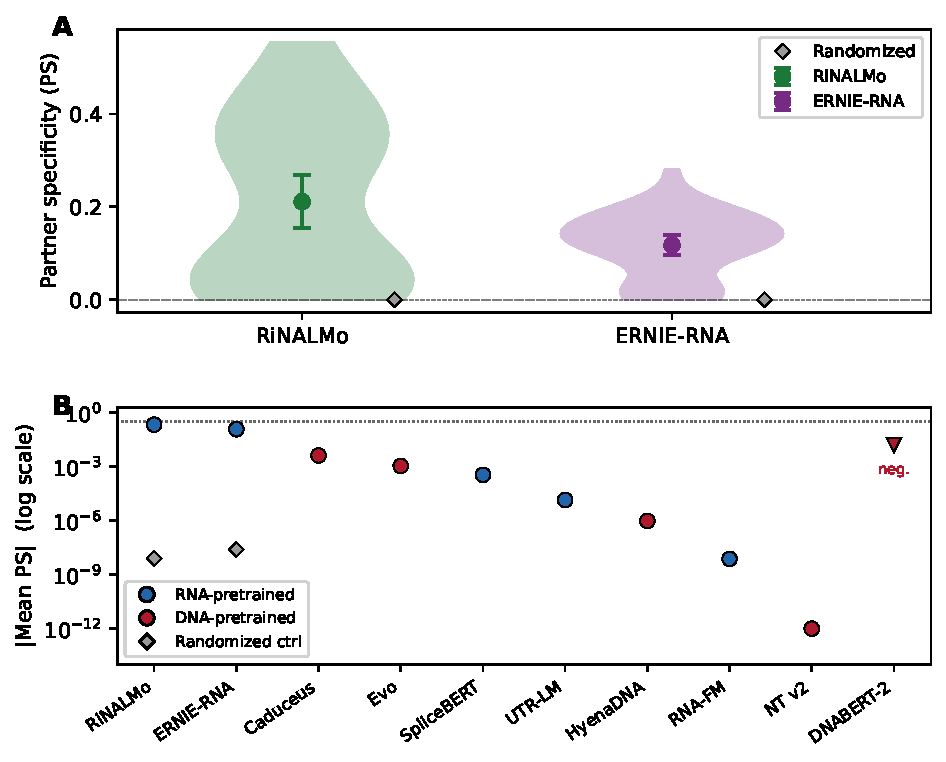
\includegraphics[width=0.85\textwidth]{../figures/figure3_partner_specificity.pdf}
\caption{Partner specificity across ten models. (A)~Per-family PS
distributions for RiNALMo and ERNIE-RNA (violins) with bootstrap 95\%
CIs (error bars); randomized-weight controls (grey diamonds) produce
PS indistinguishable from zero. (B)~$|\text{Mean PS}|$ on log scale
for all ten models, sorted by PS. RiNALMo and ERNIE-RNA exceed the
remaining models by two orders of magnitude. DNABERT-2 (negative PS)
is marked separately.}
\label{fig:ps}
\end{figure}


\subsection{The randomly initialized control}
\label{sec:random-init}

Seven models were also run with every parameter re-initialized, holding the
architecture and the tokenizer and destroying the learned weights. ERNIE-RNA's
control clears each rung of the ladder. At Rung 1 it exceeds its
composition-preserving null in 10 of $\panelN{}$ families against a chance
expectation of 2.4, retains 6 of those at Rung 2, and reaches per-pair precision
$0.490$ at Rung 3 against a chance rate of $0.241$. Judged against the
registered threshold of $1/3$ it passes, at pooled binomial $p = 2.4 \times
10^{-4}$.

The cause is a tensor that randomization does not reach.
\texttt{ErnieRnaModel} holds \texttt{pairwise\_bias\_map}, a
vocabulary-square buffer registered non-persistent, which after the first
forward pass contains six non-zero cells: A--U and U--A at $2.0$, C--G and G--C
at $3.0$, G--U and U--G at $0.8$. Re-initialization iterates a model's
parameters, and a buffer is not a parameter, so the control retains a hardcoded
Watson--Crick and wobble table while its weights are random.

% Written by scripts/generate_ablation_table.py. Do not edit.
\begin{table}[htbp]
\centering
\caption{ERNIE-RNA with and without its pairwise bias buffer, trained and
randomly initialized. Per-pair precision is the fraction of eligible pairs whose
partner is perturbed more than either of its stem neighbours. Chance is the same
fraction under a within-stem derangement, where the assigned partner is false by
construction, and excess is their difference. All four arms cover the same 35
families. Ablation zeroes \texttt{pairwise\_bias\_map} and
\texttt{pairwise\_bias\_proj} and sets the rebuild guard, without which the
first forward pass restores the buffer.}
\label{tab:ablation}
\begin{tabular}{@{}lccc@{}}
\toprule
\textbf{Arm} & \textbf{Precision} & \textbf{Chance} & \textbf{Excess} \\
\midrule
Trained, bias intact         & 0.888 & 0.124 & $+0.764$ \\
Trained, bias ablated        & 0.842 & 0.118 & $+0.725$ \\
Random-init, bias intact     & 0.490 & 0.241 & $+0.249$ \\
Random-init, bias ablated    & 0.267 & 0.255 & $+0.012$ \\
\bottomrule
\end{tabular}
\end{table}


Ablating that table and the projection above it, with the model's rebuild guard
set so the first forward pass cannot restore it, separates the two arms
(Table~\ref{tab:ablation}). Writing excess as precision minus that arm's own
chance rate, the randomly initialized model falls from $+0.249$ to $+0.012$,
while the trained model falls from $+0.764$ to $+0.725$. The difference between
those losses is $+0.198$ (95\% CI $[+0.069, +0.320]$), and the trained model's
remaining excess is $+0.725$ ($[+0.597, +0.836]$), both over
$\chanceRateN{}$ families with $\bootstrapB{}$ resamples. Predictions and
criteria were fixed before either ablated arm was computed.

Across the other nine models, one holds a buffer encoding anything about
base pairing. The rest carry position indices, rotary frequencies, or all-zero
token-type vectors, which survive randomization and encode where a nucleotide
sits rather than what it pairs with. Two randomly initialized controls
nonetheless sit above their own chance rates by $0.095$ (RiNALMo) and $0.084$
(RNA-FM), and no buffer in either accounts for it.

\subsection{Multi-sequence replication}
\label{sec:multiseq-results}

\begin{table}[htbp]
\centering
\caption{Multi-sequence replication: within-family coefficient of variation
(CV) of the stem--loop sensitivity ratio across all valid Rfam seed-alignment
sequences (51 families, 253 sequences, 3--5 per family).}
\label{tab:multiseq}
\begin{tabular}{@{}lccc@{}}
\toprule
\textbf{Model} & \textbf{Mean ratio} & \textbf{Mean CV} & \textbf{Families scored} \\
\midrule
RNA-FM     & 1.892 & 0.338 & 51/51 \\
Evo        & 1.478 & 0.244 & 51/51 \\
ERNIE-RNA  & 1.253 & 0.057 & 51/51 \\
Caduceus   & 1.203 & 0.057 & 51/51 \\
HyenaDNA   & 1.170 & 0.092 & 51/51 \\
RiNALMo    & 1.133 & 0.037 & 51/51 \\
NT~v2\textsuperscript{a} & 1.092 & 0.046 & 50/51 \\
UTR-LM     & 1.059 & 0.025 & 51/51 \\
SpliceBERT & 1.047 & 0.026 & 51/51 \\
DNABERT-2  & 0.990 & 0.100 & 51/51 \\
\bottomrule
\end{tabular}
\medskip

\small \textsuperscript{a}One Corona\_5UTR sequence excluded (numerical
overflow in ratio denominator); remaining 50 families scored normally.
\end{table}

Six models show CV $< 6$\%: UTR-LM ($0.025$), SpliceBERT ($0.026$),
RiNALMo ($0.037$), NT~v2 ($0.046$), ERNIE-RNA ($0.057$), and Caduceus
($0.057$). The stem--loop sensitivity ratio is stable across biological
replicates for these models.

RNA-FM (CV $= 0.338$) and Evo ($0.244$) show high sequence-to-sequence
variability. Both also fail composition control
(Section~\ref{sec:composition-results}), consistent with raw sensitivity
driven by sequence-specific composition rather than a stable structural
signal.


\subsection{Robustness analyses}
\label{sec:robustness}

The dinucleotide-stratified null absorbs the sole family (tRNA-Ala)
surviving the nucleotide-stratified null for RNA-FM; second-order sequence
context accounts for the residual signal. Replacing
mean aggregation with median changes PS estimates by $< 5$\% for RiNALMo
and ERNIE-RNA and does not alter the model ranking. Using the last layer
instead of the best layer reduces RiNALMo PS by 12\% and ERNIE-RNA PS by
8\%; both remain above the derangement null in $> 90$\% of gate-qualifying
families. Restricting to Watson--Crick pairs only (excluding wobble G--U
pairs) does not change the primary conclusions. Widening the PS neighbor
window from $\pm 1$ to $\pm 2$ positions reduces PS magnitudes uniformly
across models without altering their relative ranking.
A transversion control (purine $\to$ pyrimidine mutations, which
guarantee disrupted pairing) produces ratios within 1.2\% of the
Watson--Crick complement ratios for five of six models tested,
confirming that reversed base pairs differ from correct pairs enough
to register as embedding perturbations. Nine of ten
randomized-weight controls produce $|\text{PS}| < 10^{-8}$; DNABERT-2's
randomized PS ($-7.1 \times 10^{-3}$) is comparable to its trained value,
consistent with a tokenization artifact.

Family-level results and full robustness tables appear in Supplementary
Tables S2--S4.


Eight pre-registered hypotheses (SHA-256 hashed before data collection)
produced five confirmations and three failures.
The pre-registered prediction that RNA-pretrained models would
outperform DNA-pretrained models on partner specificity failed
($r_b = -0.28$, $p = 0.265$): Caduceus (14M, DNA) exceeds three RNA
models.


\subsection{Covariation versus geometry}
\label{sec:covariation-results}

Partner specificity could reflect sequence covariation rather than
learned geometric pairing. Compensatory mutations that maintain base
pairing are overrepresented in evolutionary RNA alignments; a model
trained on such sequences might predict that mutating one position
perturbs its covarying partner without encoding the physical mechanism
of pairing.

To test this, we generated synthetic sequences for each Rfam family:
the dot-bracket structure is preserved exactly, but nucleotides are
assigned randomly (uniform Watson--Crick pairs at paired positions,
uniform random at unpaired). These families share structure with their
natural counterparts but carry no evolutionary covariation.
ERNIE-RNA's mean PS drops from 0.120 (natural) to 0.035 (synthetic),
a 71\% reduction. RiNALMo drops from 0.215 to 0.061, a 71\%
reduction. Both models lose roughly 70\% of their PS when covariation
is removed. The residual synthetic PS---still orders of magnitude
above the weak-signal models---places an upper bound on the
non-covariation contribution, since the synthetic sequences also
destroy sequence context and positional composition gradients present
in natural RNA.

As an independent check, we computed mutual information (MI) between
paired positions from Rfam seed alignments (51 families, $n \geq 3$
sequences each). MI cleanly separates paired from unpaired positions
(mean MI $= 0.349$ vs $0.063$; Wilcoxon $p = 3.5 \times 10^{-10}$),
confirming that evolutionary covariation is detectable in the
alignments. Per-family mean MI does not correlate significantly with
model PS (ERNIE-RNA: $\rho = 0.320$, $p = 0.065$; RiNALMo:
$\rho = 0.265$, $p = 0.130$). Families with strong covariation signal
do not systematically produce higher PS, suggesting that the models'
partner specificity reflects learned structure rather than
recapitulated covariation.


\subsection{HTT case study}
\label{sec:htt-results}

The CAG repeat region in huntingtin exon~1 forms hairpin structures whose
stability scales with repeat count \citep{demezer2011mutant,
krzyzosiak2012triplet}. We evaluated five HTT exon~1 fragments
(NM\_002111.7) with CAG repeat counts of 17, 21, 36, 40, and 60;
structures were predicted with ViennaRNA RNAfold
\citep{lorenz2011viennarna}. Four models achieve $\geq 97$\% probing
accuracy on these predicted structures (Table~\ref{tab:htt}), but the
repeat region contains only C, A, and G---no U---creating extreme
composition bias that linear probes exploit.

\begin{table}[htbp]
\centering
\caption{HTT CAG-repeat case study. High probing accuracy coexists with null
composition-controlled signal. Attn~$\rho$: Spearman correlation between
self-attention weights and the base-pairing contact map.
Probing: linear probe accuracy for stem-vs-loop classification.
Structures are RNAfold predictions, not experimentally determined.}
\label{tab:htt}
\begin{tabular}{@{}lccccc@{}}
\toprule
\textbf{Model} & \textbf{Mean ratio} & \textbf{$>$ null} &
  \textbf{Attn $\rho$} & \textbf{Probing} &
  \textbf{WT$\to$CAG60} \\
\midrule
RNA-FM     & 1.794 & 2/5  & 0.036 & 0.813 & 0.000 \\
RiNALMo    & 1.031 & 0/5  & 0.054 & 0.985 & 0.068 \\
NT~v2      & ---$^\dagger$ & ---   & \textbf{0.140} & 0.636 & 0.013 \\
ERNIE-RNA  & 1.086 & 0/5  & 0.070 & 0.985 & 0.023 \\
SpliceBERT & 0.996 & 0/5  & 0.036 & 0.977 & 0.042 \\
UTR-LM     & 1.151 & 1/5  & 0.039 & 0.974 & 0.016 \\
\bottomrule
\end{tabular}
\medskip

\small $^\dagger$6-mer tokenization yields degenerate embeddings on
repetitive CAG. WT$\to$CAG60 = cosine distance from CAG17 reference.
\end{table}

RNA-FM produces embedding distances from wild-type below $10^{-4}$ for all
repeat counts, failing to distinguish normal from pathogenic alleles.
RiNALMo shows the strongest separation (0.068 at CAG60), with distances
increasing monotonically with repeat count. High probing accuracy on a
computationally predicted structure can coexist with null
composition-controlled signal: apparent structure decoding persists in a
strongly composition-biased context.


% ============================================================================
% DISCUSSION — 7 paragraphs
% ============================================================================
\section{Discussion}
\label{sec:discussion}

% P1: Primary conclusion + positive result
Composition-matched nulls absorb most of the apparent stem--loop
sensitivity across all ten models. Two RNA-pretrained models---RiNALMo and
ERNIE-RNA---retain reproducible partner-specific responses under the most
stringent test. Multi-sequence replication shows low within-family
variance across eight of ten models.

% P2: Why composition matching changes interpretation
The underlying problem is general: whenever a structural annotation
correlates with feature composition, any embedding metric sensitive to
feature identity inherits the correlation. The nucleotide-stratified
permutation null controls for this by breaking the structure--composition
link while preserving nucleotide identity. The same template applies to
any biological structure correlated with sequence composition.

% P3: Interpret positive models cautiously
RiNALMo and ERNIE-RNA reach partner specificity through different pathways.
ERNIE-RNA injects a base-pairing attention bias; its randomized control
shows this bias provides capacity without producing signal on its own.
RiNALMo uses standard attention without structural bias and achieves higher
PS at $7.5\times$ the parameters. Nine of ten randomized-weight controls
produce $|\text{PS}| < 10^{-8}$, supporting a learned origin; DNABERT-2's
non-negligible randomized PS ($-7.1 \times 10^{-3}$) confirms that its trained
PS reflects tokenization rather than structure. Whether
this partner specificity reflects a geometric internal model of RNA folding
or a simpler statistical regularity remains open. A synthetic
covariation control (Section~\ref{sec:covariation-results}) shows that
roughly 70\% of PS reflects evolutionary signal; the residual
$\sim$30\% provides an upper bound on learned geometric sensitivity.

% P4: What predicts composition-controlled sensitivity
Neither training domain nor architecture family alone predicts
composition-controlled sensitivity. The three SSM-based models (Evo,
Caduceus, HyenaDNA) span nearly the full range of mean ratios
(1.17--1.48), as do the seven transformers (0.99--1.89). RNA-pretrained
models occupy four of the top five positions, but Evo and Caduceus---both
DNA-pretrained---outperform three of the five RNA models. The two models
that survive the partner specificity test (RiNALMo and ERNIE-RNA) share
RNA pretraining but differ in mechanism: ERNIE-RNA injects explicit
base-pairing attention bias, while RiNALMo uses standard self-attention at
$7.5\times$ the parameters. Scale alone does not explain the result:
Evo at 7B parameters produces high raw ratios but high within-family
variance, and its signal is largely absorbed by composition nulls. What
distinguishes the two positive models from the remaining eight is an open
question whose answer likely requires internal mechanistic analysis rather
than further behavioral benchmarking.

% P5: Broader evaluation implications
RNA structure prediction benchmarks have moved toward stricter evaluation
because high apparent performance can fail to generalize across families
\citep{szikszai2022generalization}. This work extends the concern from
dataset similarity to sequence-composition confounding. NT~v2 and DNABERT-2
show near-zero embedding-level partner specificity despite passing many
families at the composition gate, suggesting that structure-relevant
information in these models, if present, may reside in attention patterns
that embedding-level metrics do not capture.

% P6: Limitations
% (Updated to reference covariation results in Section 2.5)
\paragraph{Limitations.}
The complement-swap metric tests sensitivity to single base-pair disruptions;
it does not test tertiary contacts, pseudoknots, or long-range interactions.
The synthetic covariation control (Section~\ref{sec:covariation-results})
accounts for roughly 70\% of PS, but the synthetic sequences also destroy
sequence context and positional gradients, so the residual may overestimate
true geometric sensitivity. HTT structures
are RNAfold predictions. Ten models do not cover the full model space. Pretraining-set contamination cannot be
fully reconstructed. Multi-nucleotide tokenization limits direct
comparability for NT~v2 and DNABERT-2.

\paragraph{Practical recommendations.}
Any claim that an RNA representation encodes secondary structure should
report stem--loop sensitivity alongside a nucleotide-stratified null, so
readers can separate composition sensitivity from structure awareness.
Partner specificity is more informative than aggregate stem--loop contrasts:
a model that perturbs stems more than loops may respond to GC content, while
one that selectively perturbs the annotated pairing partner encodes
positional pairing information. Randomized-weight controls should establish
each architecture's baseline capacity. Replication across
multiple sequences per family guards against single-sequence artifacts; a
coefficient of variation above 10\% signals instability. For
multi-nucleotide tokenizers, the mapping from token-level to position-level
metrics should be stated explicitly.


% ============================================================================
% MATERIALS AND METHODS (after Discussion per RNA journal format)
% ============================================================================
\section{Materials and Methods}
\label{sec:methods}

\subsection{Benchmark construction}
\label{sec:benchmark}

We evaluate \panelN{} Rfam~14.10 families \citep{kalvari2021rfam} spanning ribozymes, riboswitches, snRNAs,
cis-regulatory elements, miRNA precursors, CRISPR repeats, and other ncRNAs.
Positions are labeled stem or loop from consensus dot-bracket annotation.
Minimum inclusion criteria: $\geq 20$~nt, $\geq 5$ stem and $\geq 5$ loop
positions. Pseudoknots, noncanonical pairs, and gap positions are excluded.

All structures are consensus secondary structures from Rfam seed alignments;
none are experimentally determined crystal or cryo-EM structures. Pretraining
data overlap cannot be fully reconstructed for all models. The full family
list with accessions appears in Supplementary Table~S1.

\subsection{Models and controls}
\label{sec:models}

\begin{table}[htbp]
\centering
\caption{Models evaluated.}
\label{tab:models}
\begin{tabular}{@{}llrll@{}}
\toprule
\textbf{Model} & \textbf{Domain} & \textbf{Params} & \textbf{Architecture} & \textbf{Tokenization} \\
\midrule
RNA-FM \citep{rnafm}                    & RNA & 99M  & Transformer           & Character \\
RiNALMo \citep{rinalmo}                 & RNA & 650M & Transformer           & Character \\
ERNIE-RNA \citep{yin2024ernierna}        & RNA & 86M  & Transformer$^\dagger$ & Character \\
SpliceBERT \citep{chen2024splicebert}     & RNA & 19M  & Transformer           & Character \\
UTR-LM \citep{chu2024utrlm}             & RNA & 1.2M & Transformer           & Character \\
NT~v2 \citep{dalla2023nucleotide}        & DNA & 56M  & Transformer           & 6-mer     \\
DNABERT-2 \citep{zhou2024dnabert2}       & DNA & 117M & Transformer           & BPE       \\
Caduceus \citep{schiff2024caduceus}      & DNA & 14M  & Mamba (SSM)           & Character \\
HyenaDNA \citep{nguyen2024hyenadna}      & DNA & 5.4M & Hyena (SSM)           & Character \\
Evo \citep{nguyen2024evo}                & DNA & 7B   & StripedHyena          & Character \\
\bottomrule
\end{tabular}
\medskip

\small $^\dagger$ERNIE-RNA injects a base-pairing attention bias from the
second layer onward.
\end{table}

We evaluate ten models covering attention, SSM, and hybrid architectures
(Table~\ref{tab:models}): five pretrained on RNA, five on DNA.
Randomized-weight controls for all ten models reinitialize all
learned parameters (Xavier normal for matrices, $\mathcal{N}(0, 0.02)$
for vectors) while preserving architecture. NT~v2 and DNABERT-2 use
multi-nucleotide tokenization (6-mer and BPE), limiting direct
comparability for position-level metrics.

\subsection{Perturbation tests}
\label{sec:perturbation}

For each annotated position, we swap the nucleotide with its Watson--Crick
complement (A$\leftrightarrow$U, C$\leftrightarrow$G) and measure the cosine
distance between wild-type and mutant embeddings at that position, maximized
over layers. Cosine distance is scale-invariant across architectures.
For multi-nucleotide tokenization, token-level outputs are mapped to
nucleotide positions by distributing the token embedding equally across
constituent nucleotides.

\paragraph{Nucleotide-stratified null.}
Stem/loop labels are shuffled within each nucleotide type (1{,}000
permutations), preserving nucleotide identity while breaking its structural
label. Layer selection is repeated inside every permutation. A
dinucleotide-stratified extension additionally conditions on the 3' neighbor.

\paragraph{Partner specificity.}
\label{sec:ps-method}
For each Watson--Crick pair $(i, j)$ where $j$ is the annotated partner:
\[
\text{PS}(i,j) = \Delta_j - \max(\Delta_{j-1}, \Delta_{j+1})
\]
where $\Delta_k$ is the cosine distance at position $k$ after the complement
swap at position $i$. Positive PS indicates the model perturbs the true
partner more than its immediate neighbors (chance $= 1/3$). Partner
assignments are tested against a within-stem derangement null (500
derangements), controlling for positional and compositional confounds.

\paragraph{Covariation control.}
To distinguish learned geometric sensitivity from recapitulated evolutionary
covariation, synthetic sequences were generated for each family: dot-bracket
structure preserved exactly, nucleotides assigned randomly (uniform
Watson--Crick pairs at paired positions, uniform random at unpaired). Mutual
information (MI) between paired and unpaired positions was computed from Rfam
seed alignments as an independent covariation measure.

\subsection{Statistical analysis and replication}
\label{sec:stats}

The biological unit of replication is the RNA family. The primary outcome is
partner specificity (PS); the primary comparison is trained vs.\
randomized-weight PS. A family is \emph{gate-qualifying} for a given model
if its raw stem--loop sensitivity ratio exceeds the nucleotide-stratified
null at the 95th percentile. PS is computed only over gate-qualifying
families and aggregated as their mean.

To test stability across biological replicates, we repeat the full
evaluation on all valid sequences from Rfam~14.10 seed alignments: 253
sequences across 51 families (3--5 per family). Within-family coefficient
of variation (CV) quantifies replication stability.

Family-level bootstrap resampling (10{,}000 iterations, seed 42)
provides 95\% CIs for mean PS and mean sensitivity ratio. For the binary
gate test, each family's ratio is compared to its own 95th-percentile
permutation null; we report the count exceeding this threshold alongside
the expected false-positive count under independence
($m \times \alpha = 52 \times 0.05 = 2.6$). Bonferroni correction
($\alpha / m \approx 0.001$) provides a conservative bound.


% ============================================================================
% DATA AVAILABILITY
% ============================================================================
\section*{Data and Code Availability}

All data, scripts, and pre-registration protocols are available at
\url{https://github.com/elliottower/rna-structure-audit} and archived at
Zenodo (DOI: \href{https://doi.org/10.5281/zenodo.21362717}{10.5281/zenodo.21362717}).

The deposited panel holds one directory per model, each stamped with the commit
and library versions it was computed under. Preregistrations are frozen at a
commit hash, deviations are dated in \texttt{DEVIATIONS.md}, and reported numbers
are bound to their runs, using \texttt{prereg}, \texttt{results} and
\texttt{citations} \citep{tower2026reproducible}.


% ============================================================================
% DECLARATIONS
% ============================================================================
\section*{Acknowledgements}

The author used Claude Code \citep{anthropic2025claude} to assist with
drafting manuscript text and with writing and debugging analysis code.
The author reviewed and verified all outputs, takes full responsibility
for the accuracy and integrity of the work, and confirms that all
hypotheses, preregistered predictions, interpretations, and conclusions
are the author's own.

\paragraph{Ethics approval and consent to participate.}
This study uses exclusively publicly available pretrained model weights
and published RNA sequences. No human subjects or animal subjects were
involved. No ethical approval was required.

\paragraph{Competing interests.} The author declares no competing interests.

\paragraph{Funding.} None. This work was conducted independently.

\paragraph{Author contributions.} E.T.: Conceptualization, Methodology,
Software, Formal analysis, Investigation, Data curation, Writing ---
original draft, Writing --- review \& editing, Visualization.


% ============================================================================
% REFERENCES
% ============================================================================
\bibliographystyle{plainnat}
\bibliography{references}

\end{document}
